\myChapterParts{ПРИЛОЖЕНИЕ Б}{Результаты тестирований}

В данном приложении на рисунках 18-24 показаны результаты тестов по всем имеющимся задачам и всем имеющимся индексам. 

\par\vspace{1em}

\begin{figure}[H]
    \centering
    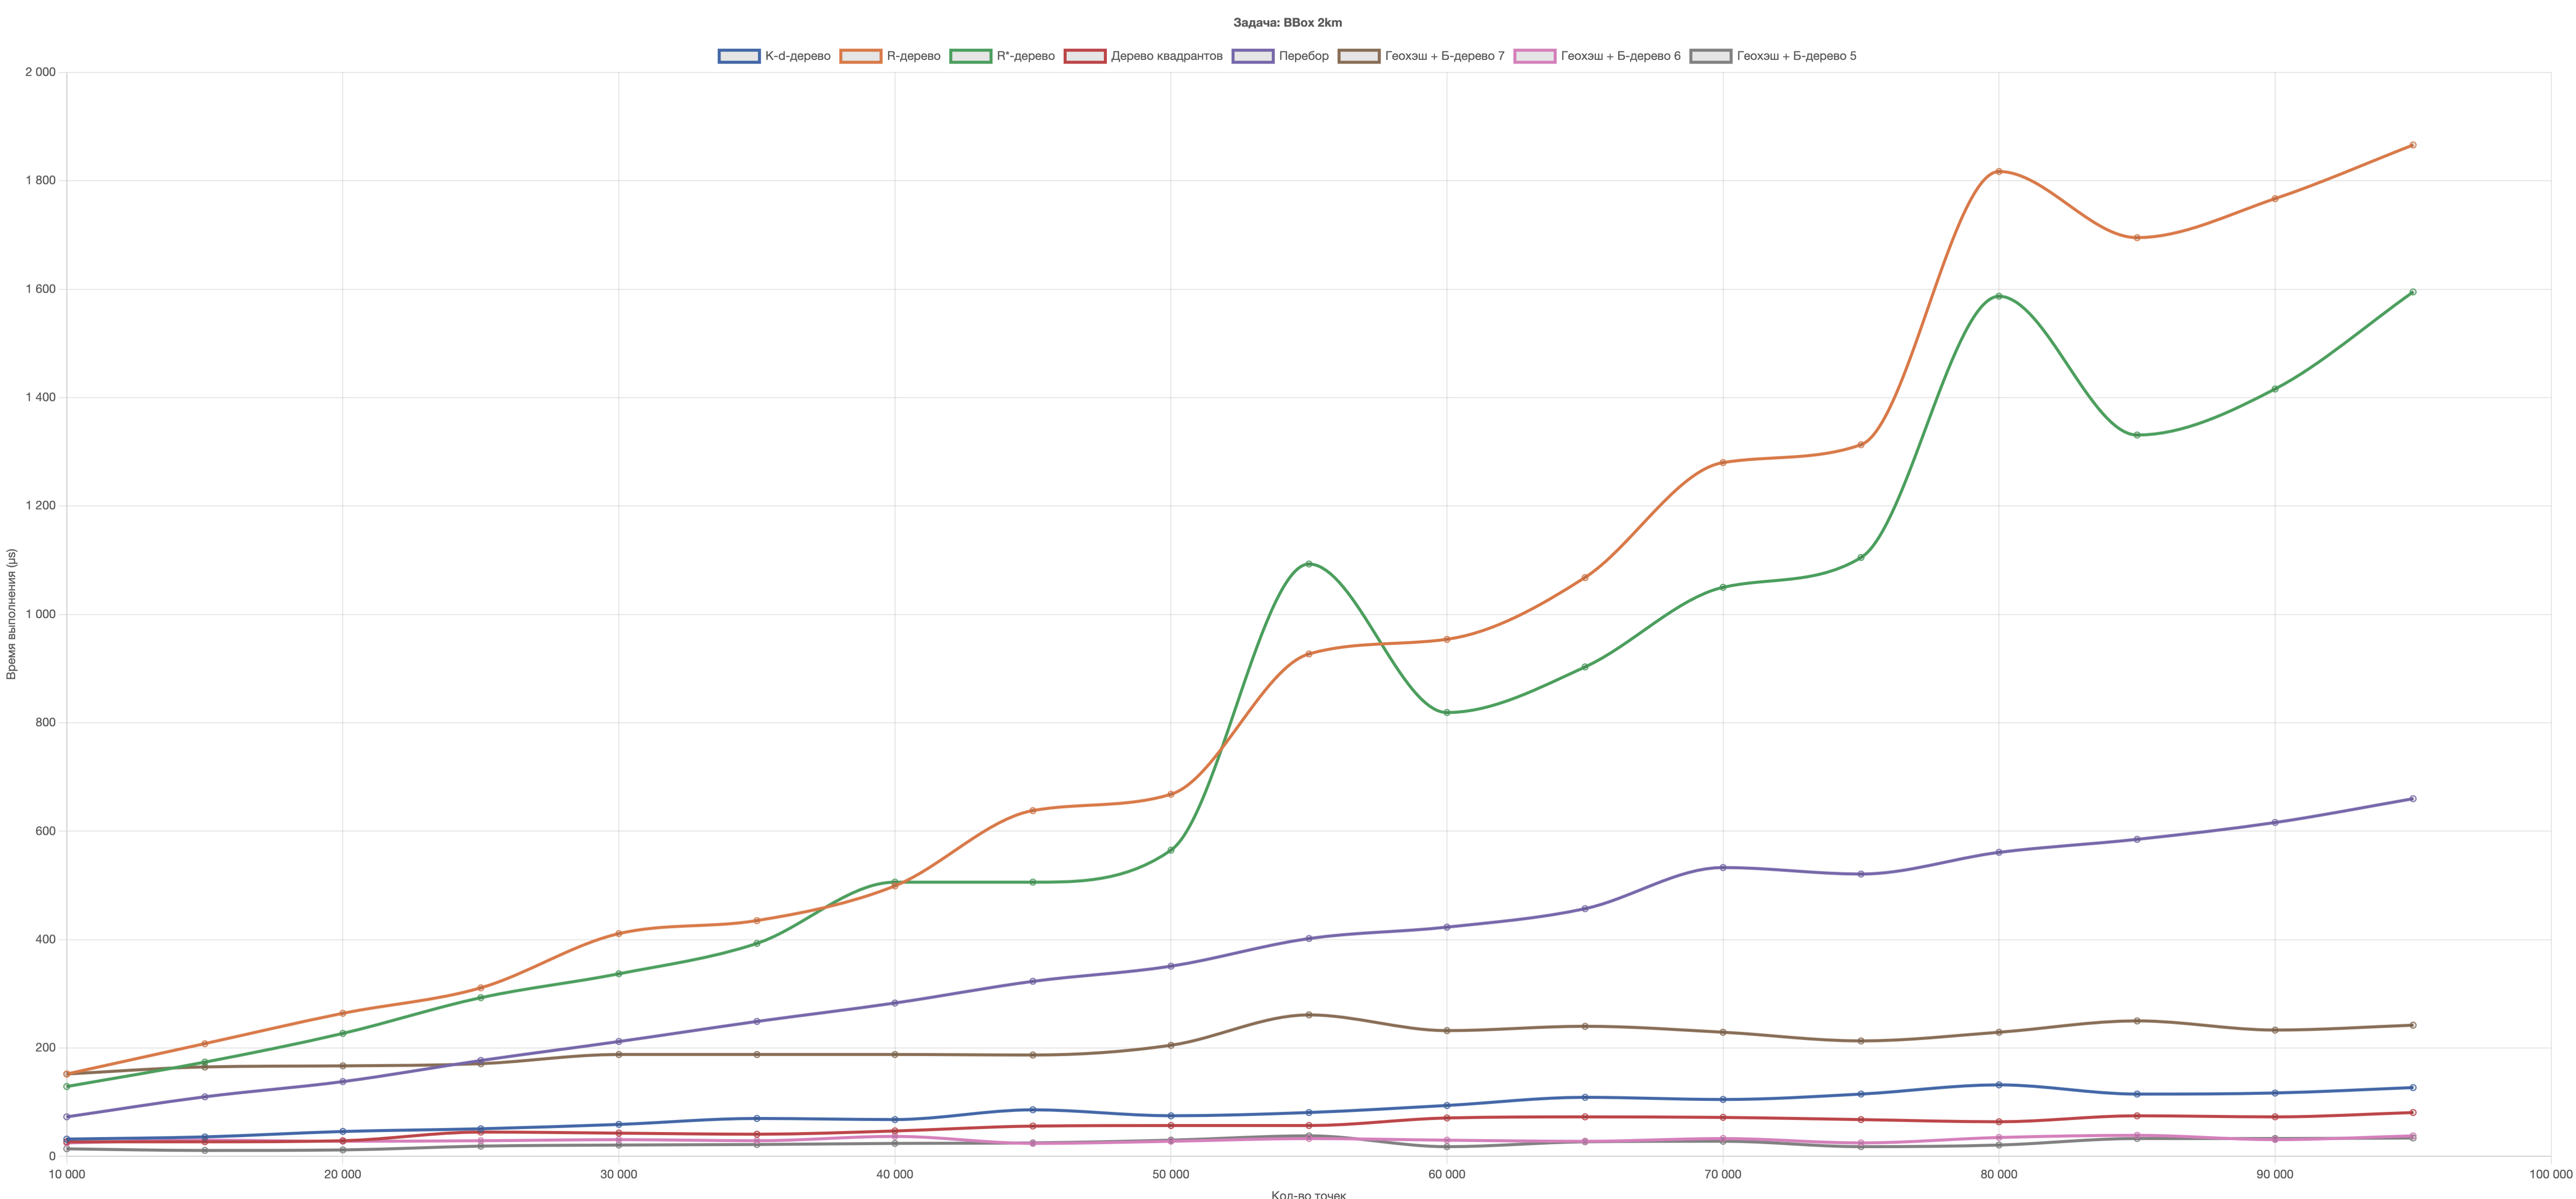
\includegraphics[scale=0.17]{results_app_1.png}
    \caption{Задача BBox на квадрате с ребром 2 км}
\end{figure}

\par\vspace{1em}

\begin{figure}[H]
    \centering
    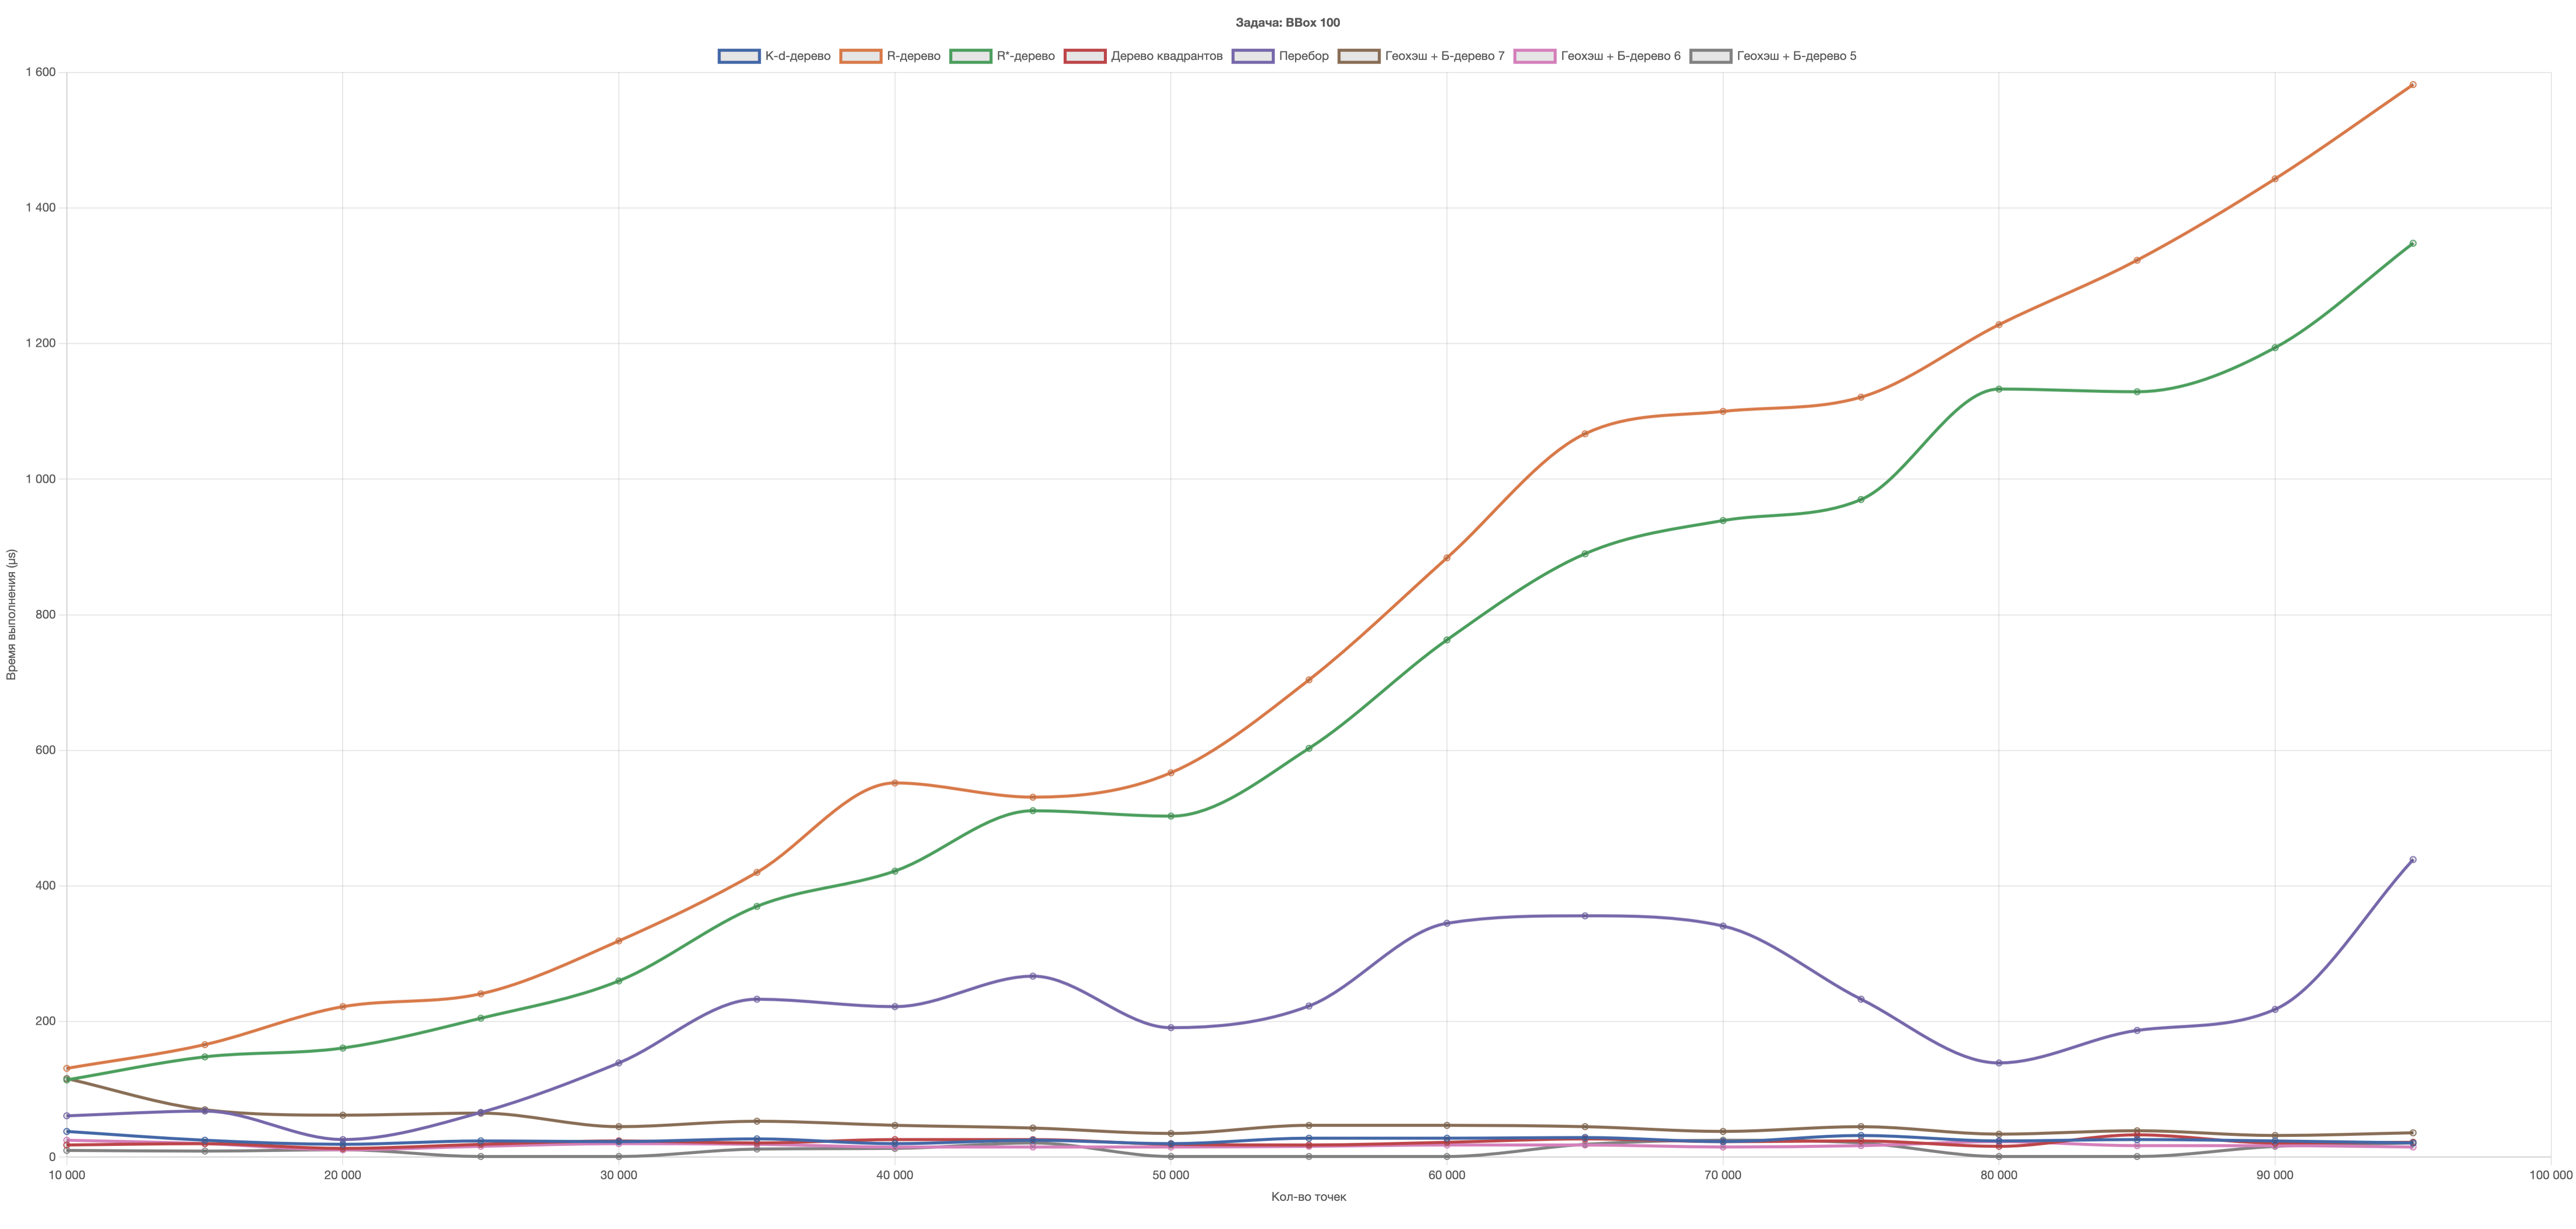
\includegraphics[scale=0.17]{results_app_2.png}
    \caption{Задача BBox на квадрате, в который входит не более 100 точек}
\end{figure}

\par\vspace{1em}

\begin{figure}[H]
    \centering
    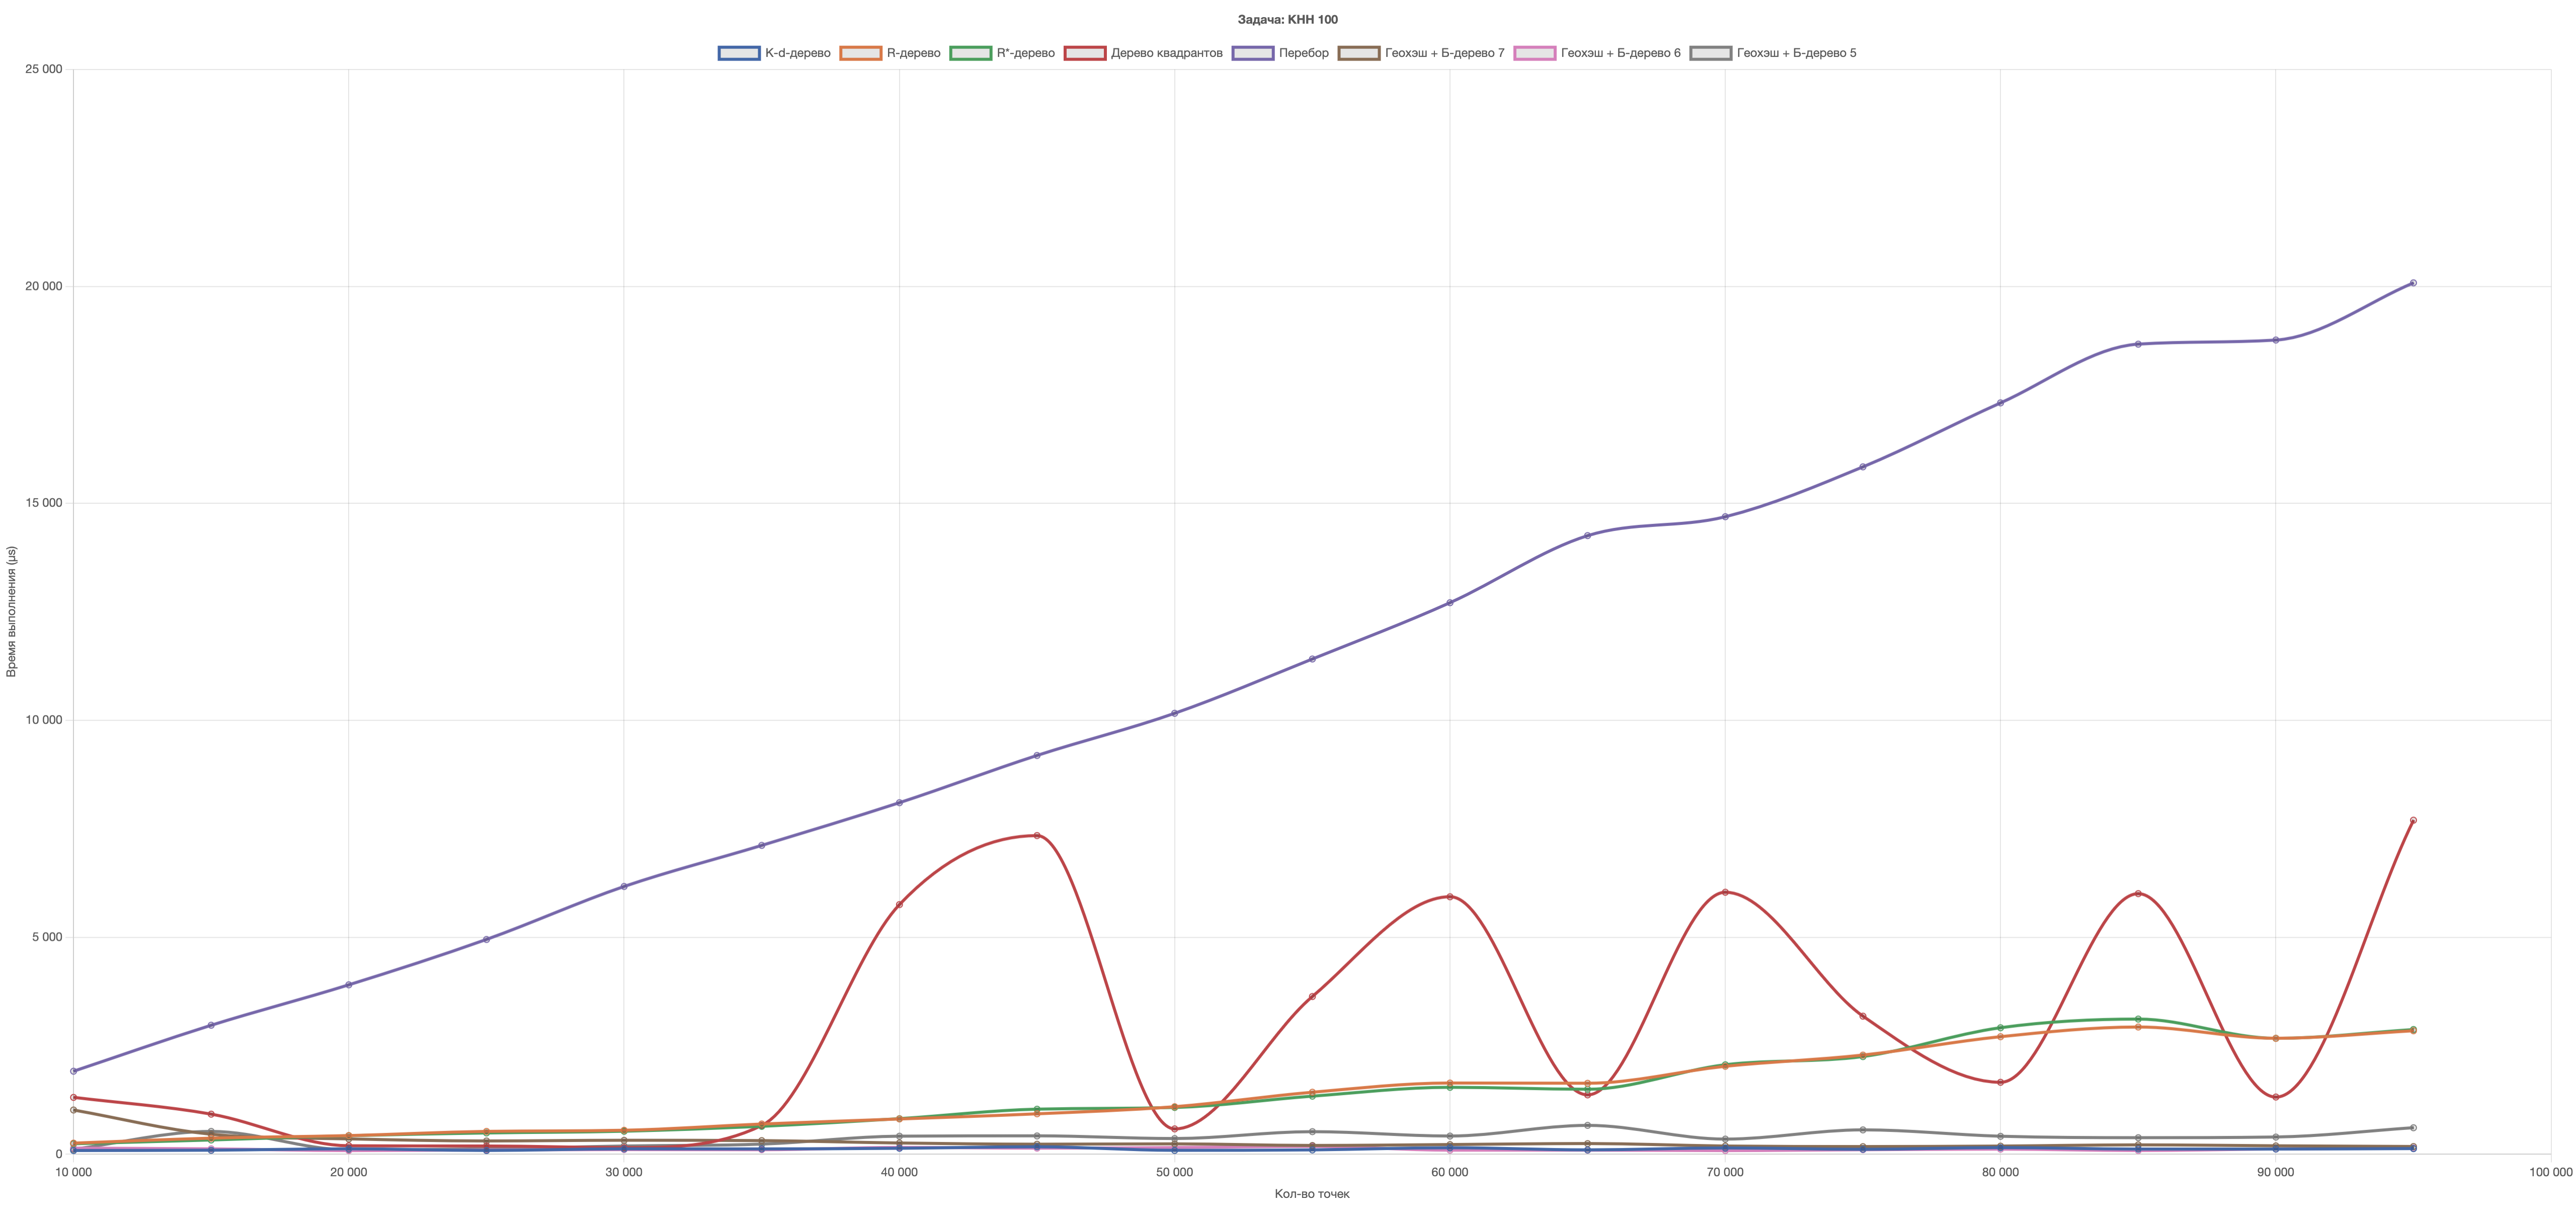
\includegraphics[scale=0.17]{results_app_3.png}
    \caption{Задача KNN на 100 точек}
\end{figure}

\par\vspace{1em}

\begin{figure}[H]
    \centering
    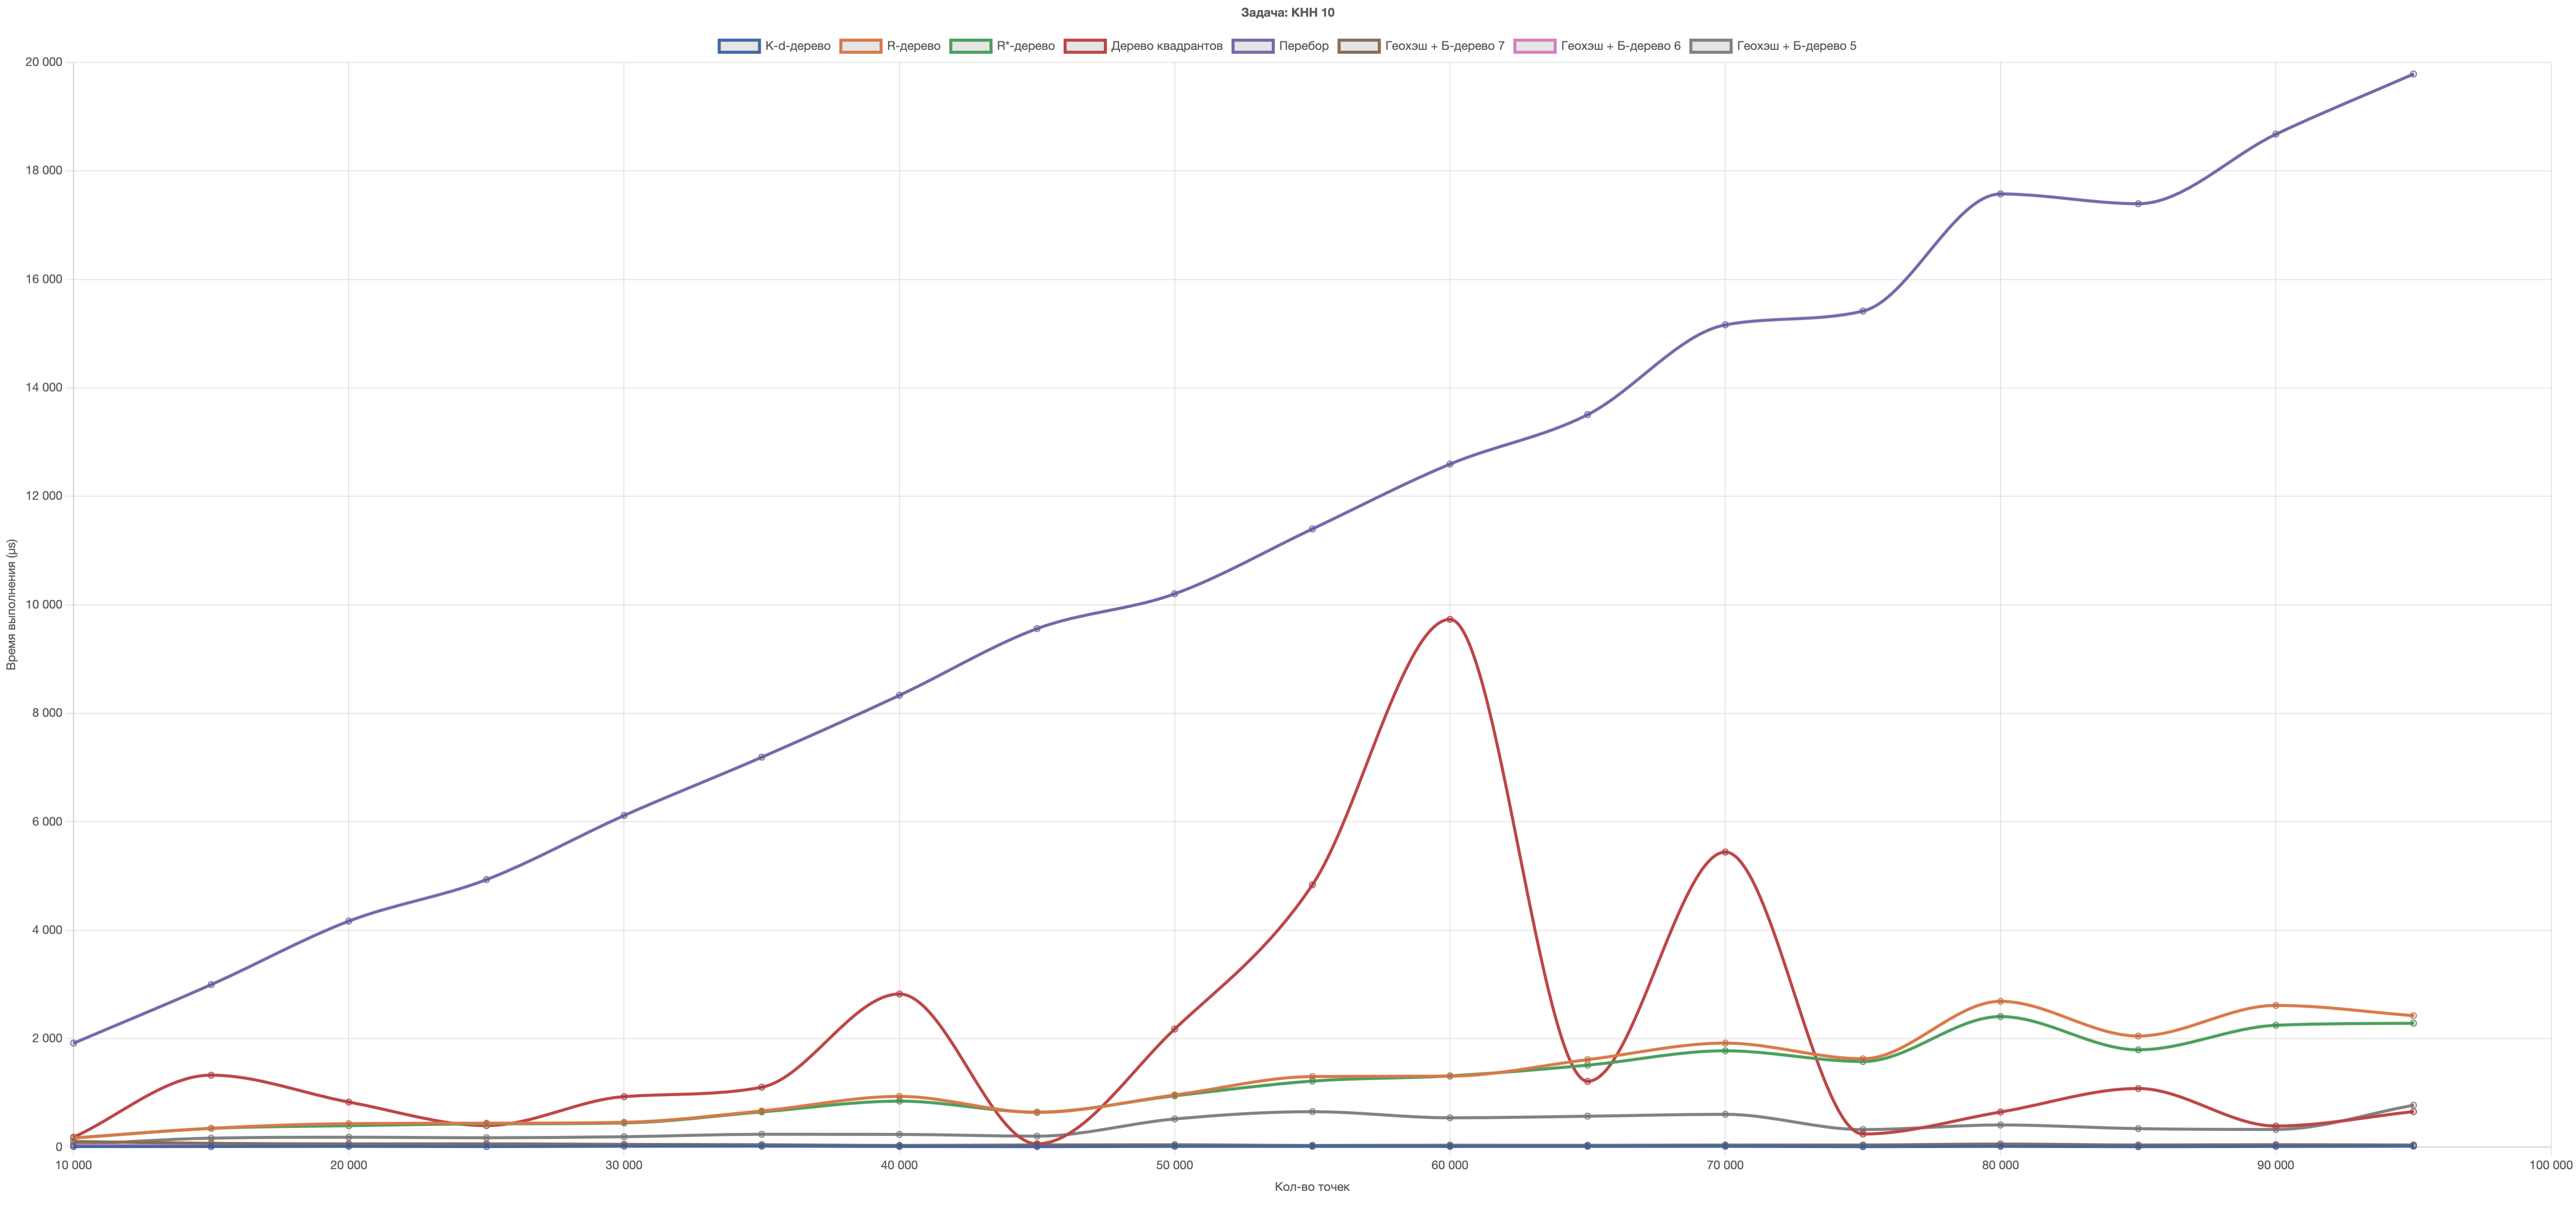
\includegraphics[scale=0.17]{results_app_4.png}
    \caption{Задача KNN на 10 точек}
\end{figure}

\par\vspace{1em}

\begin{figure}[H]
    \centering
    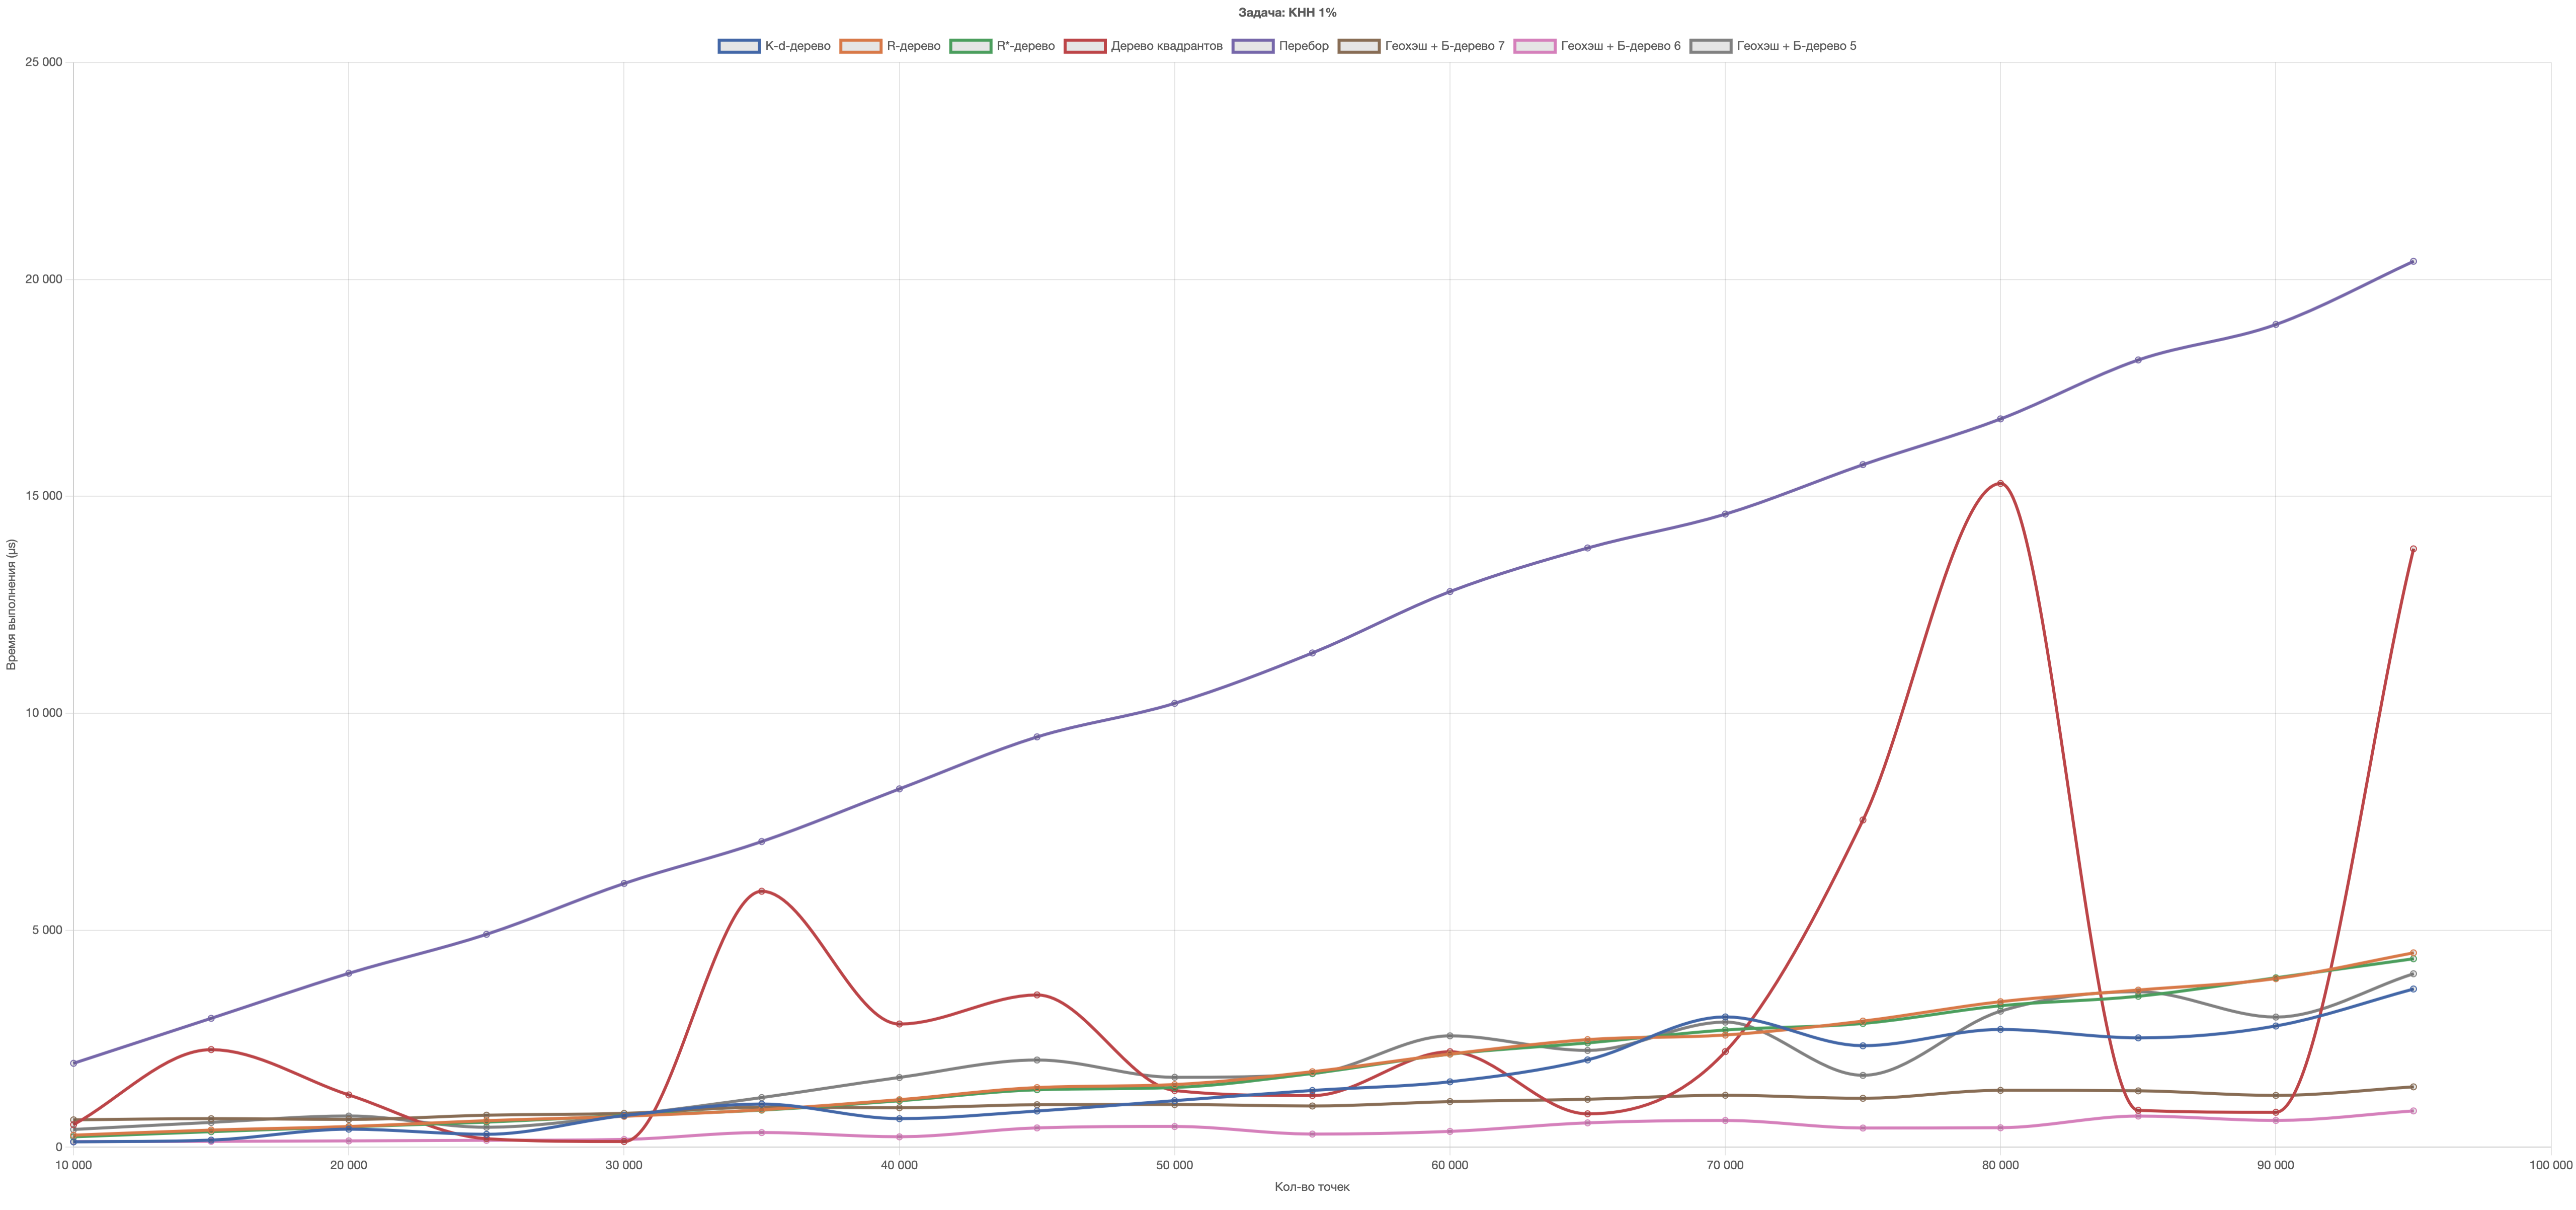
\includegraphics[scale=0.17]{results_app_5.png}
    \caption{Задача KNN на 1\% точек}
\end{figure}

\par\vspace{1em}

\begin{figure}[H]
    \centering
    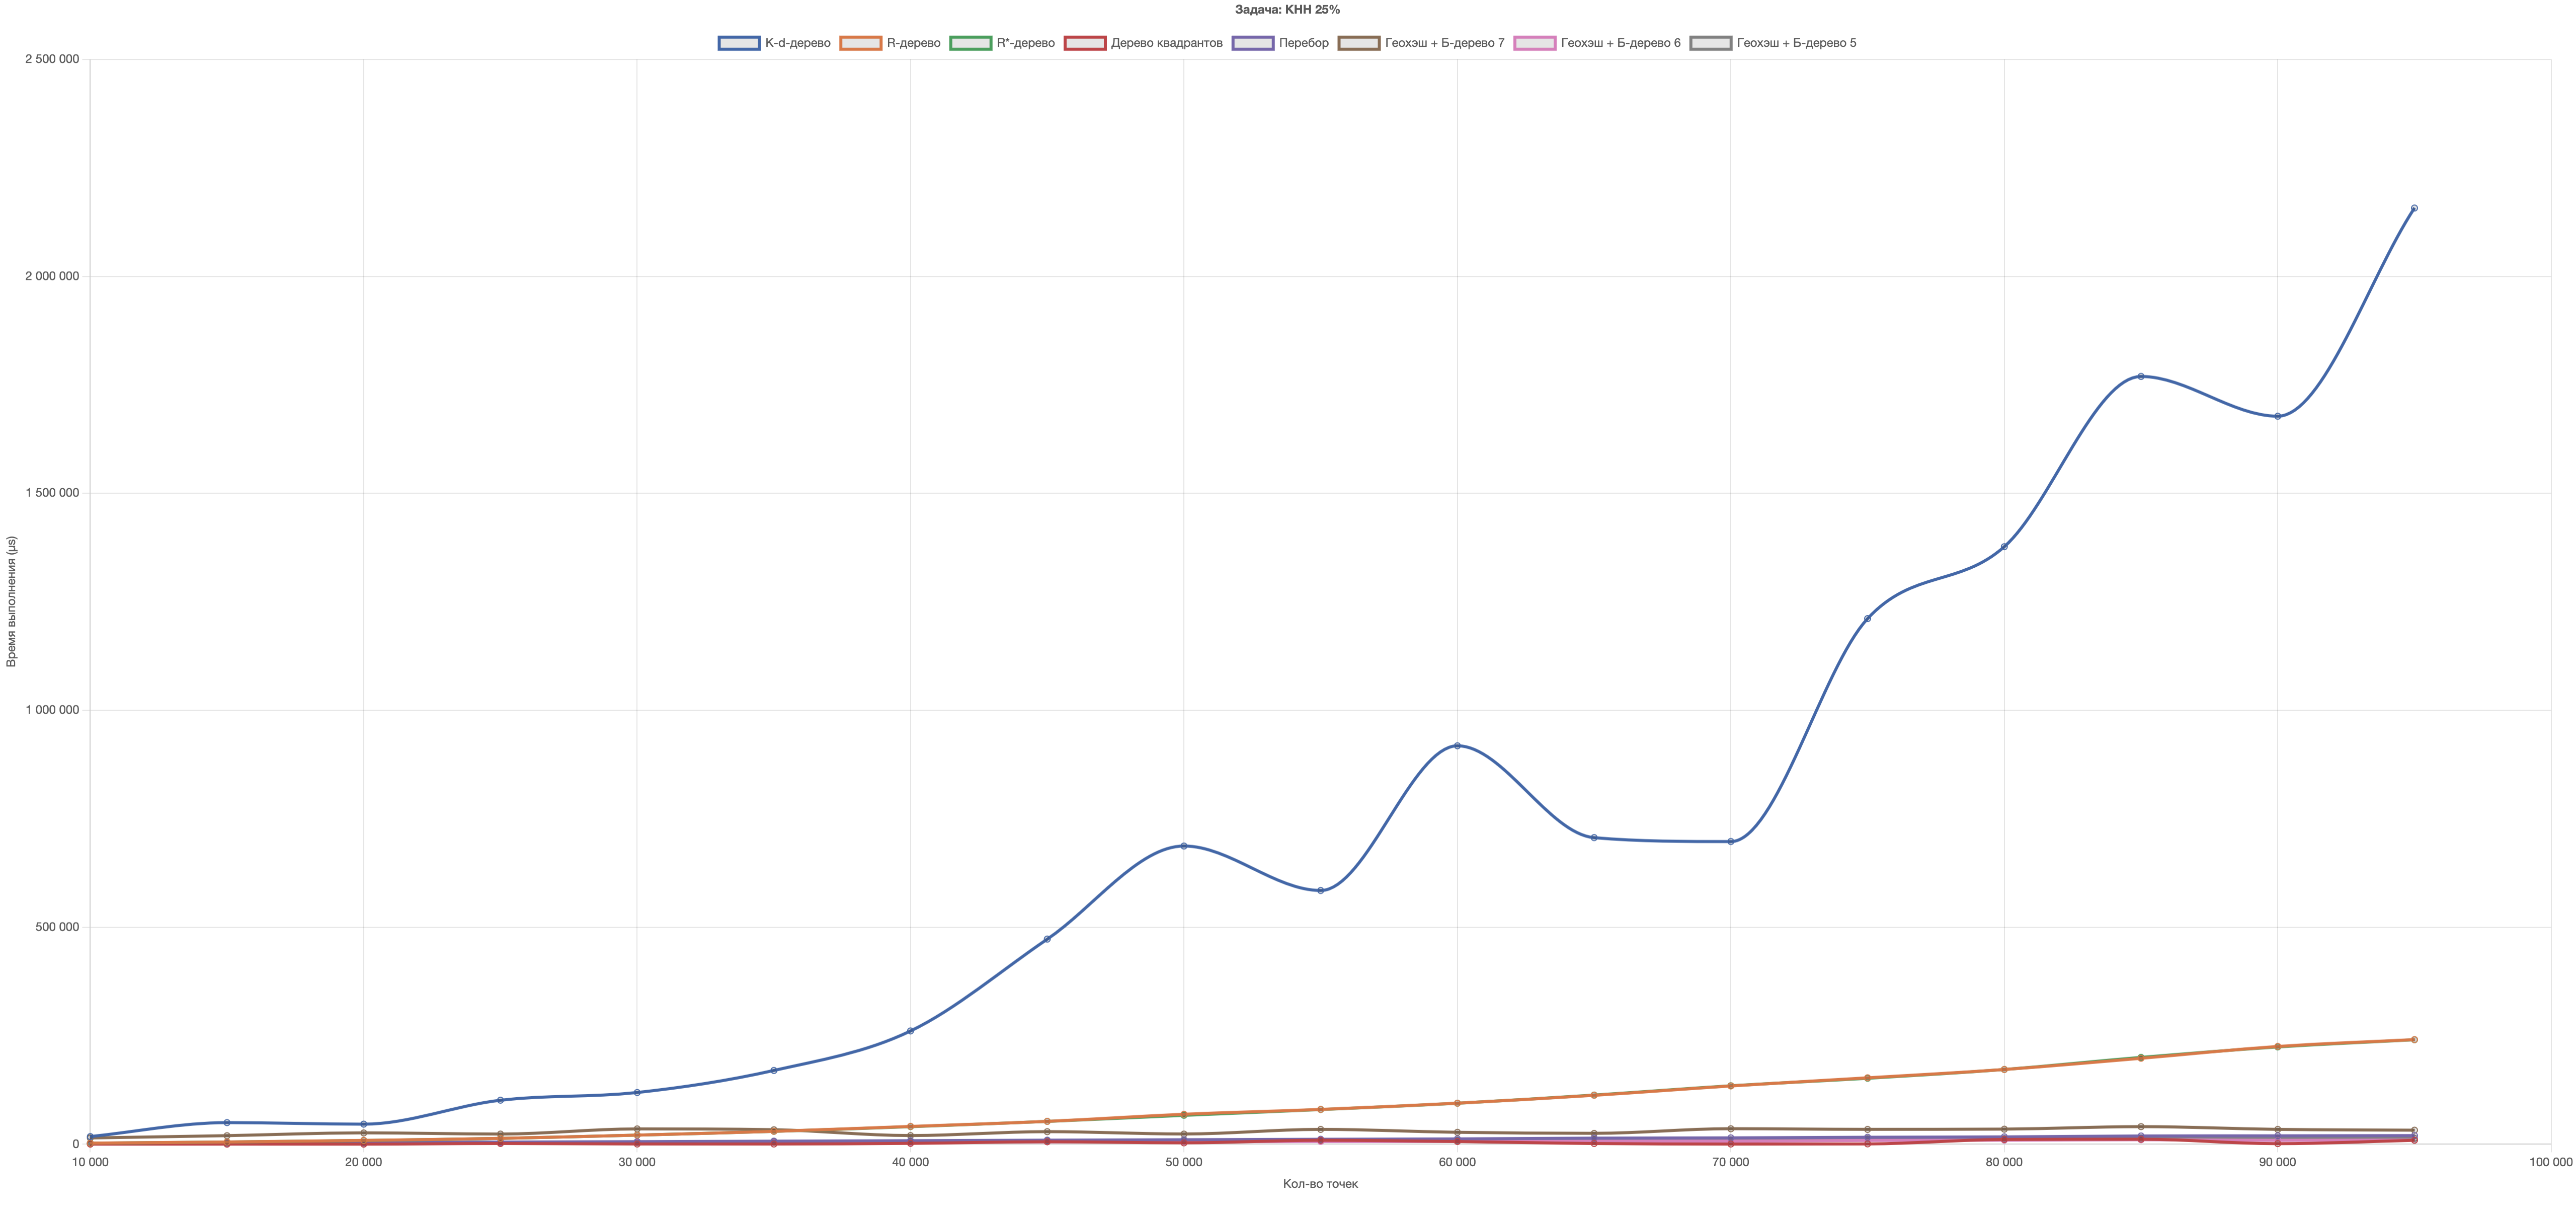
\includegraphics[scale=0.17]{results_app_7.png}
    \caption{Задача KNN на 25\% точек}
\end{figure}

\par\vspace{1em}

\begin{figure}[H]
    \centering
    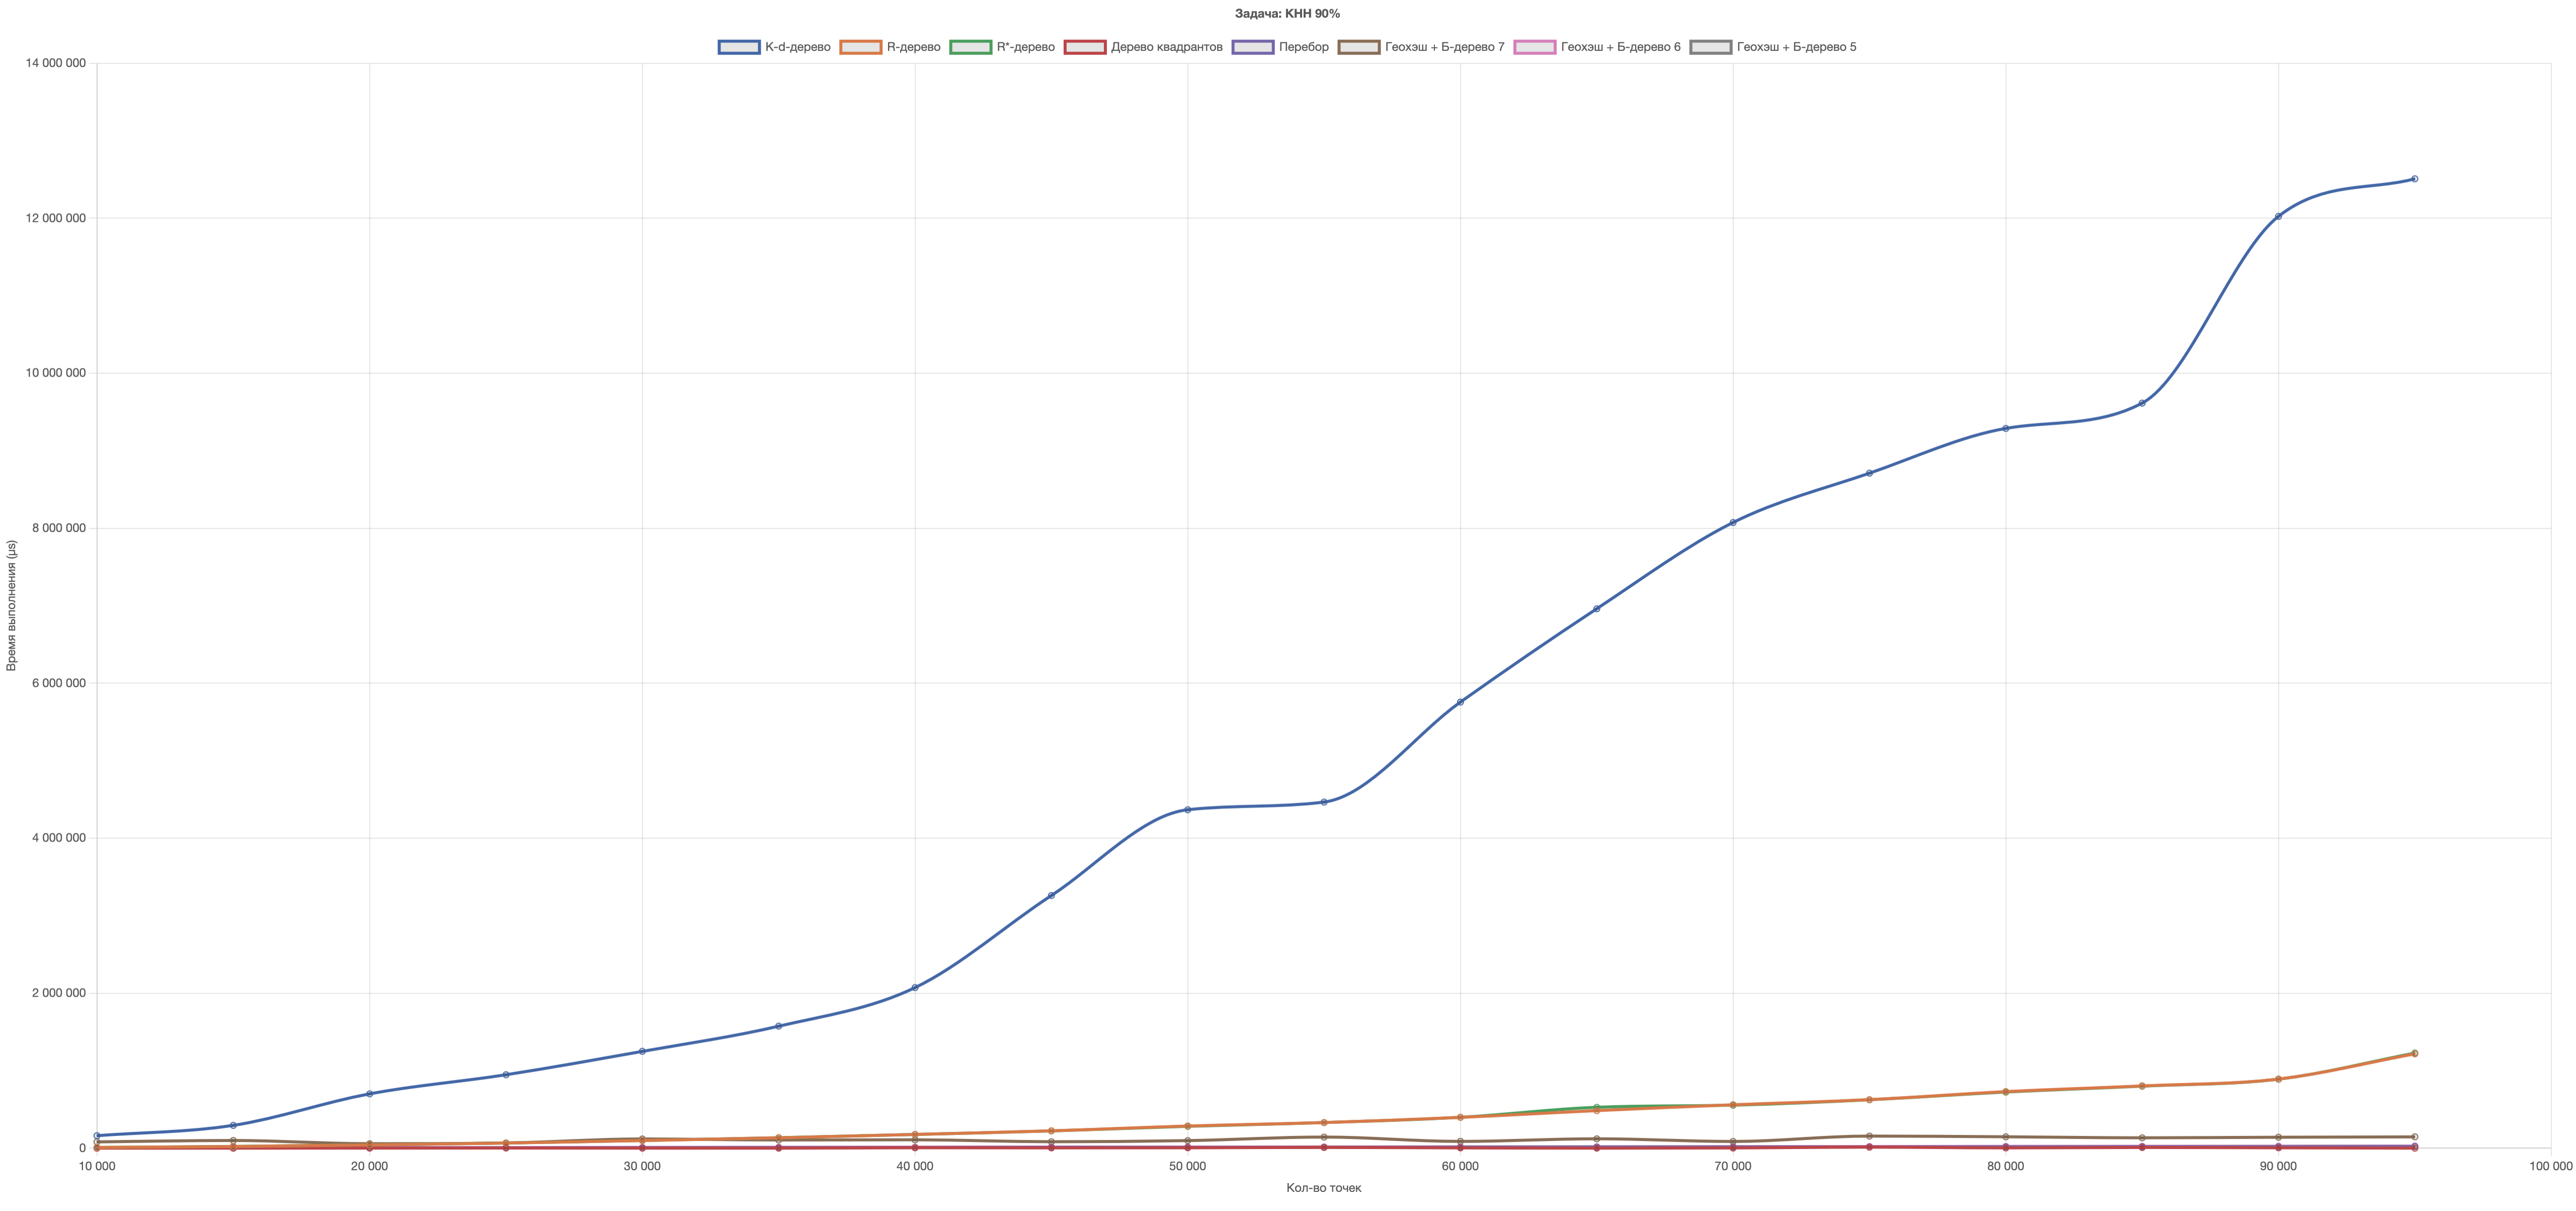
\includegraphics[scale=0.17]{results_app_6.png}
    \caption{Задача KNN на 90\% точек}
\end{figure}
